% &latex {


% %%%%%%%%%%%%%%%%%%%%%%%%%%%%%%%%%%%%%%   
% %%%%%%%%%%%%%%%%%%%%%%%%%%%%%%%%%%%%%%
\chapter{Einleitung}
\label{einleitung}



\section{Motivation und Zielsetzung}

\begin{itemize}
    \item Modellproblem mit geringerer Anzahl an freien Parametern
    \item Exploration der Möglichkeiten eines neuronalen Netzwerks
    \item Erweiterung auf Raumdimension mit verschiedenen Materialien etc.
    \item Fragestellung, ob dieses Blackbox System in Bereich der Statik wünschenswert und anwendbar ist
    \item Literaturüberblick: Was gibt es bisher? 

\end{itemize}
\subsection{Aufgabenstellung}
\begin{itemize}
    \item Verschiebungen und Spannungen an ausgewählten Punkten einer Wandscheibe in Abhängigkeit der Größe und Position der Türen und Fenster vorherzusagen
\end{itemize}

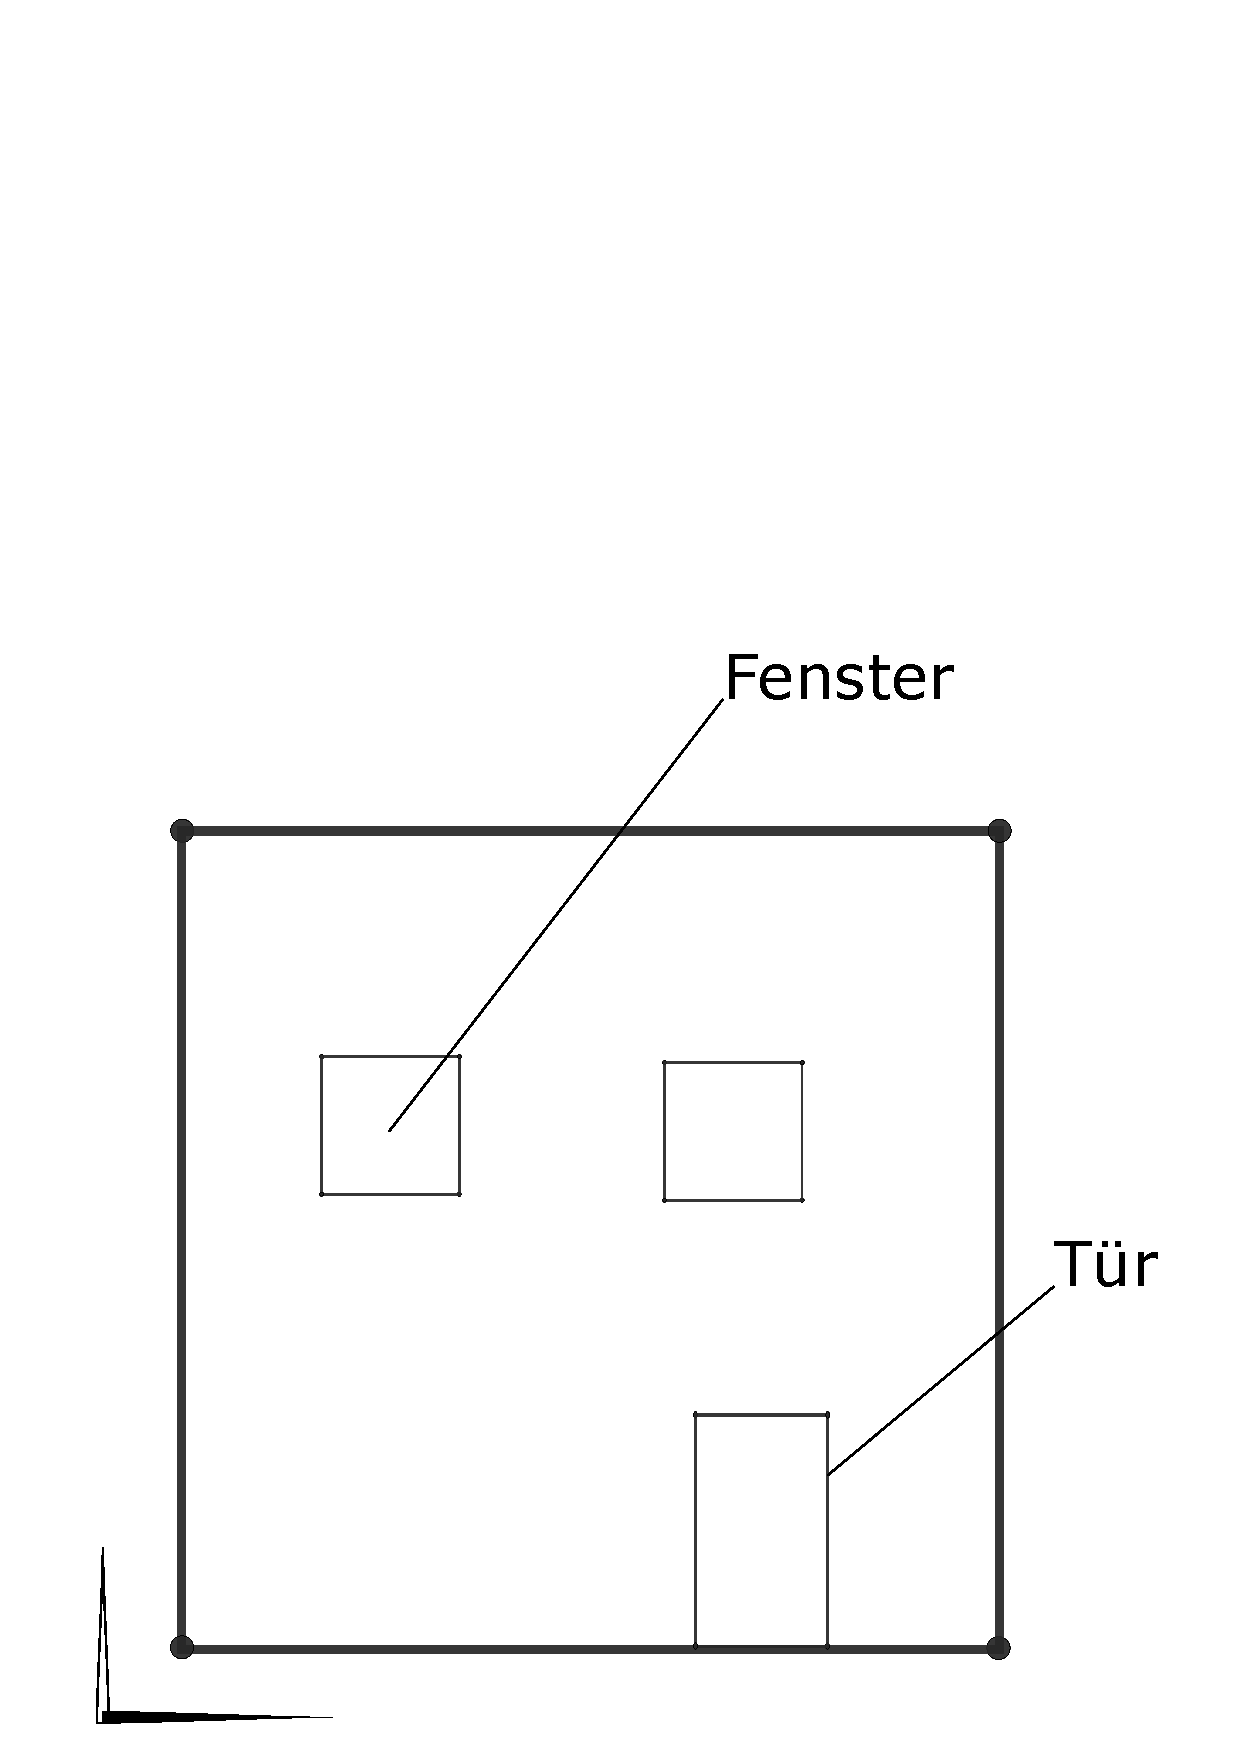
\includegraphics[width = 4cm, height = 6cm]{fig/HausGrundbau.pdf}